% =====================================================================
% Stage 4 -- Structural & Functional Design.
%
% Concrete realisations of the detailed decisions: the on-disk directory
% structure (SDS) that realises the layout decision, and the functional
% designs (FDS) -- with sequence diagrams -- that realise the eviction
% manager's reconstruction behaviour.
% =====================================================================

\begin{requirement}{SDS-LAYOUT.SHARDING-01}[draft][structuralRequirement]{Directory sharding}

  \localreqdiagram*{dsn1}{\reqid}{\reqdesc}

  Because no directory may hold more than 2,000 entries for a cache of up
  to $10^8$ objects (\reqref{REQ-EFFICIENCY.DIRSCALE-01}), each cache object
  is stored in a file named by the hexadecimal \emph{combined
  hash}\footnote{\pgsrc{pingora-cache/src/key.rs}{90}{\texttt{CacheHashKey::combined}}.}
  of the
  object's cache key (or, for a key with a user tag, by the hash described
  under \emph{User tags} below), spread across a sharded directory tree of two levels
  rather than left in one flat directory: the first-level directory is
  named after the first and second characters of the hash, and the
  second-level directory after the third and fourth characters, with the
  object file residing inside that second-level directory --- 256
  first-level directories, each holding up to 256 second-level
  directories, for 65,536 leaf directories in total. Splitting the hash
  this way, rather than keying a single level by all four characters,
  keeps every directory in the tree --- including the first-level ones ---
  at the same small entry count; a single level with the same
  65,536-bucket fan-out would instead concentrate all 65,536 buckets as
  entries in one top-level directory, itself the kind of oversized
  directory this scheme exists to avoid. The combined hash and the user tag
  are both available from the full \texttt{CacheKey} presented on lookup and
  store and from the \texttt{CompactCacheKey} presented on purge, so every
  \texttt{Storage} operation can derive an object's file --- and its shard
  --- from the key form it receives alone, with no index lookup or
  directory scan needed.

  \textbf{User tags.} A key's \texttt{user\_tag} is part of an object's
  identity, as the \texttt{pingora-cache} eviction managers count it: they key
  their entries by the whole \texttt{CompactCacheKey}, whose \texttt{Hash}
  and \texttt{Eq} cover the
  tag,\footnote{\pgsrc{pingora-cache/src/key.rs}{152}{\texttt{CompactCacheKey}}
  derives both over the primary hash, the variance, and the tag.} while the
  combined hash leaves the tag
  out.\footnote{\pgsrc{pingora-cache/src/key.rs}{220}{\texttt{CacheKey::new}}:
  ``Only the \texttt{primary} key will be hashed to produce the primary cache
  hash.''} A key with a non-empty tag is therefore named by the Blake2b-128
  hash --- the hash \texttt{pingora-cache} names keys by --- of its combined
  hash followed by the tag, in hexadecimal; a key with an empty tag keeps its
  combined hash as its name. Either way the name is 32 hexadecimal
  characters, and keys that differ only in their tag are stored, evicted, and
  purged as separate objects.

  For example, an object whose cache key hashes to \texttt{a1b2c3d4e5f6\dots} is stored at
  the path \texttt{a1/b2/a1b2c3d4e5f6\dots}: the first-level shard \texttt{a1} comes
  from characters one and two, and the second-level shard \texttt{b2} from
  characters three and four. Figure~\ref{dsn:shard-example} illustrates the layout.

  While a store is in flight, the object is written in that same
  second-level directory as a per-writer temporary, named per
  \reqref{FDS-STORAGE.PUBLISH-01} (e.g.\
  \texttt{a1/b2/a1b2c3d4e5f6\dots.4711-6fd5a44b00000001.17.tmp} for store~17
  of the backend instance holding the lease
  \texttt{writers/4711-6fd5a44b00000001.lock});
  the concluding atomic rename to the canonical name drops the suffix.
  While it grows, that temporary is also the read source for same-process
  streaming partial hits (\reqref{FRE-COMPAT.STREAMING-01}). Every object
  resides in this sharded tree for its whole lifetime, since compaction into
  aggregate files is not implemented for this version
  (\reqref{ADR-EFFICIENCY.COMPACTION-01}).

  \textbf{Meeting the bound.} The fan-out is fixed, so a leaf directory's
  entry count grows with the cache rather than being capped: with $N$
  objects hashed uniformly, each leaf holds $N/65{,}536$ objects on average,
  with a standard deviation of about $\sqrt{N/65{,}536}$. At the
  $10^8$-object capacity of \reqref{REQ-EFFICIENCY.DIRSCALE-01} that is about
  1,526 entries per leaf ($\sigma \approx 39$); the 2,000-entry bound sits
  more than twelve standard deviations above the mean, leaving room for the
  transient per-writer temporaries that share a leaf with the canonical
  names. First-level directories hold at most 256 entries each. Beyond that
  capacity the per-leaf count keeps growing with the cache; the bound is a
  design target at the stated size, not a guarantee at every size.

  \textbf{Trade-offs.} Spreading objects this way keeps per-directory
  counts small and lookups fast up to that capacity, at the cost of
  intermediate directories that must exist before an object's file can be
  created inside them --- \reqref{FDS-LAYOUT.STARTUP-01} keeps that
  existence check cheap via a cache built at construction, and a shard
  directory, once created, is never removed --- and object access that
  traverses two path components instead of one. The spread is only as
  uniform as the cache key's hash distribution; a skewed key space can
  leave some shards much larger than others.

  \begin{figure}[H]
    \centering
    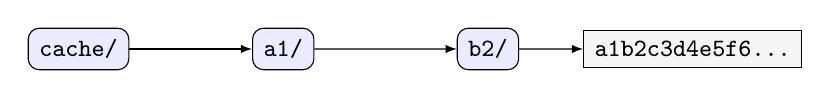
\begin{tikzpicture}[
        every node/.style={font=\ttfamily\small},
        grow=right, level distance=26mm,
        edge from parent/.style={draw, -latex},
        dir/.style={draw, rounded corners, fill=blue!8, inner sep=4pt},
        file/.style={draw, fill=gray!8, inner sep=4pt},
      ]
      \node[dir] {cache/}
        child { node[dir] {a1/}
          child { node[dir] {b2/}
            child { node[file] {a1b2c3d4e5f6\dots} }
          }
        };
    \end{tikzpicture}
    \caption{Sharded path for a cache key whose combined hash is \texttt{a1b2c3d4e5f6\dots}.}\label{dsn:shard-example}
  \end{figure}

  \reqdiaglink{global}{\textit{View complete diagram.}}

  \reqcover{verify}{TC}
  \reqcover{satisfy}{IMP}

  \refine{ADR-PERSISTENCE.MECHANISM-01}
  \satisfy{REQ-EFFICIENCY.DIRSCALE-01}
  \satisfy{FRE-COMPLIANCE.VARY-01}
  \satisfy{FRE-COMPLIANCE.VARYISOLATION-01}
  \trace{FDS-STORAGE.PUBLISH-01}
  \trace{ADR-EFFICIENCY.COMPACTION-01}
  \trace{FRE-COMPAT.STREAMING-01}

\end{requirement}

\begin{requirement}{FDS-LAYOUT.STARTUP-01}[draft][functionalRequirement]{Startup: shard directory cache}

  \localreqdiagram*{fdslayoutstartup01}{\reqid}{\reqdesc}

  \textbf{Two lifecycle moments, one cache.} The sharded tree of
  \reqref{SDS-LAYOUT.SHARDING-01} needs every shard directory to exist
  before an object's file can be created inside it. Checking that on every
  store, one file-system call at a time, is unnecessary: the tree is small
  and finite, so its existence can be established once, in memory, at
  construction, and consulted cheaply thereafter for the rest of the
  process's life, without depending on any state surviving a restart.

  \textbf{At construction.} Before the backend is handed to
  \texttt{HttpCache} as its \texttt{Storage} implementation, it shall
  ensure every first-level directory exists, creating any that are
  missing, and then, for each first-level directory, list its existing
  second-level subdirectories and record in an in-memory cache those named
  as \reqref{SDS-LAYOUT.SHARDING-01} names shards --- exactly two lowercase
  hexadecimal digits --- since anything else in the tree is not the
  backend's. This
  work is proportional only to the number of first- and second-level
  directories actually present --- at most 256 directory creations and 256
  directory listings --- never to the number of objects the cache holds,
  unlike \reqref{FDS-EVICTION.STARTUP-01}'s per-object scan. Because the
  cache is rebuilt this way at every start, it never depends on anything
  surviving a restart or a hot upgrade (\reqref{FRE-COMPAT.HOTUPGRADE-01}).

  \textbf{On each store.} A store already knows which shard its object
  belongs to (\reqref{SDS-LAYOUT.SHARDING-01}); the first-level directory
  is guaranteed to exist by construction, so only the second-level
  directory needs a decision. The backend shall consult the in-memory
  cache before creating an object's file: if the shard is already known,
  it proceeds directly; if not, it creates the second-level directory ---
  tolerating a concurrent store that reaches the same new shard first ---
  and adds it to the cache before proceeding. Because
  \reqref{SDS-LAYOUT.SHARDING-01} never removes a shard directory once
  created, the cache is purely additive: entries are only ever added, so
  none ever needs to be invalidated or re-checked against the file system.
  Something outside the backend may still remove a directory: IF creating a
  store's temporary fails because a shard directory the cache records as
  existing is missing, THEN the backend shall create that directory again
  and retry the creation once, and return a second failure as the store's
  error (\reqref{FRE-COMPAT.WRITEFAIL-01}).

  \textbf{Concurrency.} \texttt{Storage} is called from multiple threads at
  once (\reqref{FRE-COMPAT.CONCURRENT-01}), so the cache shall be safe for
  concurrent reads and inserts. Inserting an already-present shard shall be
  a harmless no-op --- two stores racing to create the same new shard both
  succeed, and both insertions land safely. The whole
  second-level namespace is small enough to track exactly, without
  approximation: a bitset over all 65,536 possible shards
  (\reqref{SDS-LAYOUT.SHARDING-01}) needs only 8~KiB.

  \begin{figure}[H]
    \centering
    \begin{adjustbox}{max width=\textwidth}
    \begin{sequencediagram}
      \newinst[0.0]{Integrator}{\guillemotleft actor\guillemotright\ Integrator}
      \newinst[0.5]{Storage}{Storage}
      \newinst[2.2]{DirectoryCache}{DirectoryCache}
      \newinst[0.5]{FileSystem}{File System}
      \begin{sdalt}{strict}{[at construction]}
        \begin{call}{Integrator}{new()}{Storage}{}
          \begin{call}{Storage}{mkdir() (each of 256 first-level dirs)}{FileSystem}{}
          \end{call}
          \begin{call}{Storage}{readdir() (each first-level dir)}{FileSystem}{existing shards}
          \end{call}
          \begin{call}{Storage}{insert(existing shards)}{DirectoryCache}{}
          \end{call}
        \end{call}
      \sdpart{[on each store, once traffic begins]}
        \begin{call}{Storage}{contains(shard)?}{DirectoryCache}{known / unknown}
        \end{call}
        \begin{call}{Storage}{mkdir(shard) if unknown (tolerate EEXIST)}{FileSystem}{}
        \end{call}
        \begin{call}{Storage}{insert(shard) if unknown}{DirectoryCache}{}
        \end{call}
      \end{sdalt}
    \end{sequencediagram}
    \end{adjustbox}
    \caption{Shard-directory cache: built once at construction by scanning
    the existing tree, then consulted (and grown) on each store. The
    \emph{strict} fragment marks its two regions as strictly sequential ---
    construction always completes before the backend is handed to
    \texttt{HttpCache}.}\label{fig:fds-layout-startup-seq}
  \end{figure}

  \reqdiaglink{global}{\textit{View complete diagram.}}

  \reqexpect{verify}{TC-LAYOUT.DIRCACHE-01}{Verify the cache is rebuilt
  accurately from disk at every construction, and that concurrent
  first-time stores into the same shard never fail or double-create.}
  \reqcover{satisfy}{IMP}

  \refine{SDS-LAYOUT.SHARDING-01}
\end{requirement}

\begin{requirement}{SDS-LAYOUT.OBJECTFILE-01}[draft][structuralRequirement]{Object-file record layout}

  \localreqdiagram*{dsn2}{\reqid}{\reqdesc}

  Each cache object is persisted as one self-describing \emph{record} --- the
  internal layout of the single file of \reqref{ADR-STORAGE.OBJECTFILE-01}. The
  record has four parts, in file order
  (Figure~\ref{dsn:singlefile-strip}): a fixed-size \emph{record header}, the
  object's serialised
  \texttt{CompactCacheKey}\footnote{\pgsrc{pingora-cache/src/key.rs}{153}{\texttt{struct CompactCacheKey}}.},
  a \emph{metadata region} of
  recorded capacity holding the object's two metadata segments plus free
  headroom for their growth, and the body bytes.

  \textbf{Metadata exactly as \texttt{pingora-cache} hands it over.} A
  \texttt{CacheMeta} serialises to two opaque byte segments --- the
  \emph{internal metadata} (the framework's created/updated instants,
  freshness deadline, and variance hash, MessagePack-encoded) and the
  \emph{header metadata} (status, protocol version, and header fields in the
  framework's own header encoding) --- and is rebuilt by
  \texttt{CacheMeta::deserialize(internal, header)}; the stock
  \texttt{MemCache} keeps precisely this pair per object. The record stores
  the same two segments byte for byte and never parses or edits them, so the
  round-trip fidelity duties on header fields and freshness inputs
  (\reqref{FRE-COMPLIANCE.HEADERS-01}, \reqref{FRE-COMPLIANCE.FRESHNESS-01})
  are met by construction: lookup returns what store received.

  \textbf{Record header: one aligned block.} The record header is a single
  44-byte block at offset~0, written and read as one unit: every field is a
  fixed-width little-endian integer at a naturally aligned offset (the
  \texttt{u64} at offset~8, every other field a \texttt{u32} at a multiple
  of four), so the block is saved by writing an
  in-memory \texttt{\#[repr(C)]} struct's bytes verbatim and read back by
  reading the block straight into that struct --- no field-by-field parsing,
  and byte swapping only on a big-endian host, as each field is read or
  written. No byte is spent on
  alignment filler: \texttt{version} and \texttt{key\_len} are each a
  \texttt{u32} rather than the \texttt{u16} their own range would need, so
  they close the gap that natural alignment would otherwise leave before
  \texttt{body\_len} and \texttt{internal\_len} respectively, instead of
  leaving it as unnamed padding. A future format revision that needs more
  header fields is free to define a different layout under a new
  \texttt{version}; nothing here is reserved against that in advance.
  Figure~\ref{dsn:singlefile-header} shows the byte placement; the fields are:
  \begin{itemize}
    \item \texttt{magic} (u32, offset 0) and \texttt{version} (u32, offset 4):
      identify the record format and its revision, so a scan can recognise
      records and a later revision can evolve the layout. \texttt{magic} is
      the four bytes \texttt{PDCR} (the little-endian value
      \texttt{0x52434450}); this layout is \texttt{version}~1. The version is
      the backend's own: it changes whenever records written before would no
      longer be read back exactly --- a change to this layout, or a
      \texttt{pingora-cache} release whose metadata encoding differs
      (\reqref{FRE-COMPAT.FORMATUPGRADE-01}) --- and a reader treats a record
      of any other version as a miss. Version~0 marks a record
      \emph{withdrawn} because its metadata outgrew the region (below), and
      is never a format version.
    \item \texttt{body\_len} (u64, offset 8): the body's exact byte length,
      patched at store completion.
    \item \texttt{meta\_capacity} (u32, offset 16): the byte size of the
      metadata region as allocated in \emph{this} record.
    \item \texttt{key\_len} (u32, offset 20): the length of the serialised
      \texttt{CompactCacheKey}, which is not constant across records: only
      \texttt{primary} (16 bytes) is
      fixed-size,\footnote{\pgsrc{pingora-cache/src/key.rs}{154}{\texttt{primary:
      HashBinary}} is a \texttt{[u8; 16]}.} while
      \texttt{variance}\footnote{\pgsrc{pingora-cache/src/key.rs}{156}{\texttt{variance:
      Option<Box<HashBinary>>}}: absent for a key with no \texttt{Vary}
      variant, 16 bytes when present.} is present or absent per key and
      \texttt{user\_tag}\footnote{\pgsrc{pingora-cache/src/key.rs}{157}{\texttt{user\_tag:
      Box<str>}}, ``the len should be small to keep memory usage bounded''
      per its own source comment --- guidance, not a fixed width.} is an
      arbitrary-length string; \texttt{key\_len} is what lets a reader
      locate the metadata region without assuming a size. The key segment's
      encoding is \reqref{SDS-LAYOUT.KEYSEGMENT-01}'s.
    \item \texttt{internal\_len} (u32, offset 24) and \texttt{header\_len}
      (u32, offset 28): the current lengths of the two metadata segments.
    \item \texttt{meta\_crc} (u32, offset 32): CRC-32C over the key and the
      two metadata segments.
    \item \texttt{body\_crc} (u32, offset 36): CRC-32C over the body's
      \texttt{body\_len} bytes, recorded at store completion
      (\reqref{ADR-PERSISTENCE.DURABILITY-01}); zero in a build without the
      \texttt{body-crc} feature. A reader never checks a stored zero.
    \item \texttt{header\_crc} (u32, offset 40): CRC-32C over header bytes
      0--39.
  \end{itemize}
  Every checksum in the record uses CRC-32C (the Castagnoli polynomial).

  \textbf{Segment placement.} The key segment starts immediately after the
  header, at offset 44, and the metadata region immediately after the key,
  with no padding: every segment is read into its own buffer, never
  interpreted in place, so none needs alignment. The region holds the
  internal and header segments back-to-back, followed by free headroom. Its capacity is fixed when the
  record is created --- the combined size of the segments actually presented
  (there is no fixed cap, so an arbitrarily large header set simply yields a
  larger region, \reqref{FRE-COMPLIANCE.HEADERS-01}) plus the configured
  growth headroom (\reqref{FDS-STORAGE.METAUPDATE-01}), a deployment setting
  defaulting to 512 bytes. The capacity is
  \emph{recorded} in \texttt{meta\_capacity}, so a reader computes the body
  offset (44 + \texttt{key\_len} + \texttt{meta\_capacity}) from the record
  alone and records written under
  different configurations coexist. The body follows, to the end of the file.

  \textbf{Why the key is stored.} The file is \emph{named} by the combined
  hash (\reqref{SDS-LAYOUT.SHARDING-01}), which cannot be inverted back to the
  key, while eviction admissions and purges are keyed by the
  \texttt{CompactCacheKey}.\footnote{\pgsrc{pingora-cache/src/eviction/mod.rs}{252}{\texttt{EvictionManager::admit}}
  takes a \pgsrc{pingora-cache/src/eviction/mod.rs}{53}{\texttt{CacheEntryKey}} and
  \pgsrc{pingora-cache/src/storage.rs}{194}{\texttt{Storage::purge}} a
  \pgsrc{pingora-cache/src/storage.rs}{51}{\texttt{PurgeTarget}}; both are thin
  wrappers that carry a \texttt{CompactCacheKey} and, for a backend that assigns
  them, an entry identifier this backend does not
  (\reqref{ADR-COMPAT.ENTRYID-01}). The key each needs is therefore the same
  \texttt{CompactCacheKey}.} The key segment is what lets the startup scan of
  \reqref{FDS-EVICTION.STARTUP-01} recover \texttt{admit(key, size,
  fresh\_until)} for every persisted entry --- the key from the key segment,
  the size as the record's file length (the record size
  \reqref{FRE-COMPAT.EVICTION-01} defines), the freshness deadline from the
  deserialised metadata --- reading only the header, key, and metadata region,
  never the body (\reqref{FRE-COMPAT.EVICTION-01}). It also lets any
  reader confirm a record matches the key it looked up, catching a
  wrong-shard read caused by a software defect or on-disk corruption, and
  lets the restart scan reclaim a record found anywhere but at its own key's
  path (\reqref{FDS-STORAGE.RECLAIM-01}).

  \textbf{A weaker collision guard than it looks.} That confirmation is not
  a defence against a genuine hash collision for every key: a key with
  neither a variance nor a user tag has \texttt{CompactCacheKey}'s
  \texttt{primary} field exactly equal to the combined hash that named its
  file (\reqref{SDS-LAYOUT.SHARDING-01}), so two different keys
  colliding there would carry identical stored keys too and go undetected.
  Only a varianced key gets a real check, because its stored
  \texttt{primary} and \texttt{variance} survive as the separate values
  they were before \texttt{combined\_bin} folded them together
  (\reqref{SDS-LAYOUT.SHARDING-01}) --- a collision in that folding step is
  independent of a collision in either value alone. No comparable cache
  pays for a stronger guarantee across the board: the stock
  \texttt{MemCache} trusts the combined hash as its map key with no
  comparison at
  all,\footnote{\pgsrc{pingora-cache/src/memory.rs}{313}{\texttt{MemCache::lookup}}
  looks an object up by \texttt{key.combined()} alone --- whatever is
  stored under that hash is returned unconditionally.} and Traffic
  Server's on-disk record stores only hashes of the key, never the
  original URL, so its own read-time check is exactly as hash-bound as
  this one.\footnote{\texttt{first\_key} and \texttt{key} are both a
  \texttt{CryptoHash}, never the request URL itself.
  \href{https://github.com/apache/trafficserver/blob/10.1.4/src/iocore/cache/P_CacheDoc.h\#L45-L49}{Apache
  Traffic Server source (release 10.1.4):
  \texttt{src/iocore/cache/P\_CacheDoc.h}, lines 45--49}.} Keying storage
  on the full, unhashed request string instead --- as Caddy's Souin-based
  cache module does\footnote{\href{https://github.com/darkweak/souin/blob/v1.7.8/context/key.go\#L147}{Souin
  source (release v1.7.8): \texttt{context/key.go}, line 147} builds the
  storage key by concatenating the method, scheme, host, path, query, and
  varied header values verbatim, never folding them into a fixed-size
  hash.} --- would remove the question entirely, at the cost of storing,
  and comparing on every lookup, a full request string that is typically
  far longer than the 16-byte hashes this record carries.

  \textbf{Write, publication, and integrity.} The header, key, and metadata
  region are written when the store's miss handler
  opens\footnote{\pgsrc{pingora-cache/src/storage.rs}{176}{\texttt{Storage::get\_miss\_handler}}
  hands the backend the \texttt{CacheMeta} directly, before any body bytes
  arrive.} --- the
  \texttt{CacheMeta} is available then; body
  chunks are appended as they stream in, each folded into a running CRC-32C
  kept in memory unless the build leaves out the \texttt{body-crc} feature.
  While the per-writer temporary grows
  (\reqref{SDS-LAYOUT.SHARDING-01}), the valid length lives in the in-memory
  in-flight registry that backs streaming partial hits
  (\reqref{FDS-STORAGE.PARTIAL-01}); the on-disk header is \emph{not}
  the source of truth for readers of an in-flight write. At completion the
  backend patches \texttt{body\_len} and \texttt{body\_crc}, recomputes
  \texttt{header\_crc}, synchronises the file's data to stable storage, and
  renames the temporary to the canonical name
  (\reqref{FDS-STORAGE.PUBLISH-01}, \reqref{ADR-PERSISTENCE.DURABILITY-01}).

  A reader accepts a published record only if, in this order: the magic and
  \texttt{version} match this layout's; \texttt{header\_crc} verifies; the
  metadata segments fit within \texttt{meta\_capacity}; the computed body
  offset lies within the file; \texttt{meta\_crc} verifies (with the
  re-reads described under in-place updates below); the stored key equals the
  looked-up key; and the file's length is \emph{exactly} the computed body
  offset plus \texttt{body\_len}. The two bounds come before the reader
  sizes any read by a length the header carries, so no header, however
  forged, makes it allocate or read beyond the file. Any failure --- a truncated
  file, a torn or foreign record --- makes the lookup report a miss, so a
  damaged record is never served (\reqref{FRE-COMPLIANCE.INCOMPLETE-01}). The
  reader does not remove the file: a later store of the same key replaces it,
  and the restart-time scan reclaims it (\reqref{FDS-STORAGE.RECLAIM-01}),
  so a lookup never unlinks a path whose content may have changed since it
  opened it. A reader does not check the body against \texttt{body\_crc}:
  integrity at rest is the storage layer's
  (\reqref{ADR-PERSISTENCE.DURABILITY-01}). A build with the
  \texttt{body-crc-verify} feature can switch a check on in its
  configuration: a reader that streams the whole body from its start then
  computes CRC-32C over the bytes it delivers and, at the end, compares it
  with \texttt{body\_crc}; on a mismatch it logs an error naming the file and
  still ends the stream normally, since every byte has already been
  delivered. A published record supports seeking: its hit handler reports
  \texttt{can\_seek}, and a seeked read delivers exactly the requested slice
  (\reqref{FRE-COMPLIANCE.BODY-01}) and is never checked, since the checksum
  covers only a whole body. Figure~\ref{fig:sds-objectfile-lookup-seq}
  shows the read path this validation belongs to.

  \begin{figure}[H]
    \centering
    \begin{adjustbox}{max width=\textwidth}
    \begin{sequencediagram}
      \newinst[0.0]{HttpCache}{HttpCache}
      \newinst[3.7]{Storage}{Storage}
      \begin{call}{HttpCache}{lookup(key)}{Storage}{(CacheMeta, HitHandler) / None}
        \postlevel
        \postlevel
        \postlevel
        \begin{callself}{Storage}{{\small \shortstack{no in-flight write for the key (\reqref{FDS-STORAGE.PARTIAL-01});\\compute combined hash (\reqref{SDS-LAYOUT.SHARDING-01});\\open file at shard path; read 44-byte header}}}{}
        \end{callself}
        \begin{sdalt}{alt}{[magic, version, CRCs, key, and length all valid]}
          \postlevel
          \begin{callself}{Storage}{{\small \shortstack{deserialise CacheMeta from internal + header segments}}}{}
          \end{callself}
        \sdpart{[any single check fails --- damaged, incomplete, or foreign]}
          \postlevel
          \begin{callself}{Storage}{{\small treat as a miss; leave the file}}{}
          \end{callself}
        \end{sdalt}
      \end{call}
      \begin{sdalt}{loop}{[on a hit: read\_body() until exhausted]}
        \begin{call}{HttpCache}{read\_body()}{Storage}{chunk / None at EOF / error}
          \postlevel
          \postlevel
          \begin{callself}{Storage}{{\small \shortstack{read the next slice from the validated body offset}}}{}
          \end{callself}
        \end{call}
      \end{sdalt}
    \end{sequencediagram}
    \end{adjustbox}
    \caption{Lookup/read sequence for a published record (an in-flight write
    of the key is served first, as \reqref{FDS-STORAGE.PARTIAL-01}
    specifies): the reader recomputes the file's own path from the key,
    opens it, and validates the record before trusting it. Any single
    validation failure --- a bad magic or version, a CRC mismatch, a
    different stored key, or a length that is not exactly
    the computed body offset plus \texttt{body\_len} --- is indistinguishable
    from any other: the lookup reports a miss and leaves the file for a later
    store or the restart-time scan
    (\reqref{FRE-COMPLIANCE.INCOMPLETE-01}, verified by
    \reqref{TC-LAYOUT.OBJECTFILE-01}). On a hit, the already-validated file
    stays open and every \texttt{read\_body} call simply advances through
    it; unlike Figure~\ref{fig:fds-publish-seq}'s concurrent
    \texttt{Follower}, this reader never races a body append, since the
    file it opened was already published at open time (an in-place
    metadata update may still race the metadata read, handled by the
    re-reads described below).}\label{fig:sds-objectfile-lookup-seq}
  \end{figure}

  \textbf{Metadata updates in place.} A metadata update
  (\reqref{FRE-COMPLIANCE.REVALIDATION-01}) whose new segments fit
  \texttt{meta\_capacity} --- the reserved headroom decided in
  \reqref{FDS-STORAGE.METAUPDATE-01} --- is applied in place: the segments
  are rewritten in the region, then \texttt{internal\_len},
  \texttt{header\_len}, and the CRCs are updated --- the body is never
  touched --- and nothing is synchronised to stable storage
  (\reqref{ADR-PERSISTENCE.DURABILITY-01}). A reader that catches the update
  mid-write sees a CRC mismatch and re-reads the header and metadata region,
  up to three more times, yielding to other tasks between attempts. If all
  four reads mismatch --- the updater may have been stopped between its two
  writes --- the lookup reads once more holding the key's publication lock
  (\reqref{FDS-STORAGE.METAUPDATE-01}), which every metadata update holds
  from its first write to its last, so that this read finds the record
  whole. Only if that read mismatches too does the lookup report a miss and
  leave the file, as for any damaged record; the restart scan reads such a
  record once more in the same way before it reclaims it
  (\reqref{FDS-STORAGE.RECLAIM-01}). A reader therefore observes
  the pre- or post-update set, never a mixture, and an update in progress
  never turns a hit into a miss. This assumes nothing about the write itself being atomic ---
  no POSIX filesystem or disk interface guarantees that a multi-byte write
  lands as one indivisible unit, even for a single nominal sector or
  page,\footnote{\href{https://www.sqlite.org/atomiccommit.html}{SQLite
  documentation: ``Atomic Commit In SQLite''}: ``SQLite has traditionally
  assumed that a sector write is not atomic.''} the metadata region can
  exceed any one write unit once the header set is large enough (there is
  no fixed cap on it), and the update spans two separate byte ranges ---
  the metadata region and the header block's own length fields --- that no
  single write covers together regardless. Treating this as a live, not
  theoretical, risk matches established practice: PostgreSQL's
  \texttt{full\_page\_writes} exists because ``a page write that is in
  process during an operating system crash might be only partially
  completed, leading to an on-disk page that contains a mix of old and new
  data,''\footnote{\href{https://www.postgresql.org/docs/18/runtime-config-wal.html\#GUC-FULL-PAGE-WRITES}{PostgreSQL
  18 documentation: \texttt{full\_page\_writes}}.} and MySQL's InnoDB
  doublewrite buffer exists for the identical reason, recovering a good
  copy when a crash lands ``in the middle of a page
  write.''\footnote{\href{https://dev.mysql.com/doc/refman/8.0/en/innodb-doublewrite-buffer.html}{MySQL
  8.0 Reference Manual: ``Doublewrite Buffer''}.} A cheaper-looking
  alternative --- marking the record \emph{writing} before the update and
  \emph{done} after, so only the rare writer pays a check instead of every
  reader --- does not remove the requirement: without an explicit ordering
  barrier between the status write and the payload write, the file system
  is free to persist them out of order --- \texttt{fsync} only flushes
  ``modified in-core data\ldots{} to the disk device,'' so anything not yet
  flushed simply sits reorderable in the page cache until it
  is,\footnote{\href{https://man7.org/linux/man-pages/man2/fsync.2.html}{Linux
  manual page: \texttt{fsync(2)}}.} and a crash could therefore leave a
  durable \emph{done} status covering a payload that never actually
  landed. Enforcing that ordering costs at least one synchronous flush per
  write --- PostgreSQL's own documentation calls exactly this delay ``a
  major component of the total transaction time'' for short transactions,
  the reason its asynchronous-commit mode exists at
  all,\footnote{\href{https://www.postgresql.org/docs/current/wal-async-commit.html}{PostgreSQL
  documentation: ``Asynchronous Commit''}.} typically millisecond-scale on
  hardware without power-loss
  protection\footnote{\href{https://smalldatum.blogspot.com/2026/01/ssds-power-loss-protection-and-fsync.html}{Mark
  Callaghan, ``Small Datum'': ``SSDs, power loss protection and fsync
  latency''}: consumer SSDs measured at roughly 1--5~ms per
  \texttt{fsync}, versus under 0.1~ms for enterprise drives with
  power-loss protection.} --- far more than the microsecond-scale check it
  would replace. Nor is the read-side check adding a separate cost to
  shift in the first place: \texttt{CacheMeta::deserialize} already needs
  the whole internal and header byte range in memory to decode it, so the
  CRC recompute is one more pass over bytes already resident from the read
  that just happened, not a second read or a meaningfully separate
  computation.

  \textbf{Metadata that outgrows the region.} When the new metadata no
  longer fits \texttt{meta\_capacity}, the record is \emph{withdrawn}
  instead (\reqref{FDS-STORAGE.METAUPDATE-01}): only its header is
  rewritten, with \texttt{version}~0 and \texttt{header\_crc} resealed.
  Every reader then treats the key as holding no object, so the next request
  fetches it again, and its store, sized for the new metadata, replaces the
  file; until then the file keeps its length, and the space the eviction
  manager counts for it. The body is neither read nor moved, and a reader
  that catches the header write midway sees a checksum or version mismatch
  and ends with the record whole or a miss, never a mixture. The reserved
  headroom is what makes the common freshening after a \texttt{304}
  (\texttt{Date}- and \texttt{Age}-scale changes) an in-place write rather
  than a withdrawal and a fetch from the origin. Moving outgrown metadata
  after the body instead, which would spare that fetch, is deferred to a
  later version (\reqref{ADR-STORAGE.METAMOVE-01}).

  \textbf{Self-delimiting for future reuse.} The record is self-delimiting ---
  header, key length, capacity, and body length define its exact extent.
  Object compaction into shared aggregate files is not implemented for this
  version (\reqref{ADR-EFFICIENCY.COMPACTION-01}); this property is what
  would let a future version move a completed record verbatim, back-to-back
  with others, into an aggregate without redesigning it, and let such an
  aggregate be re-scanned sequentially --- for recovery or startup
  enumeration --- without a separate index.

  \begin{figure}[H]
    \centering
    \begin{subfigure}{\textwidth}
      \centering
      \begin{adjustbox}{max width=\textwidth}
      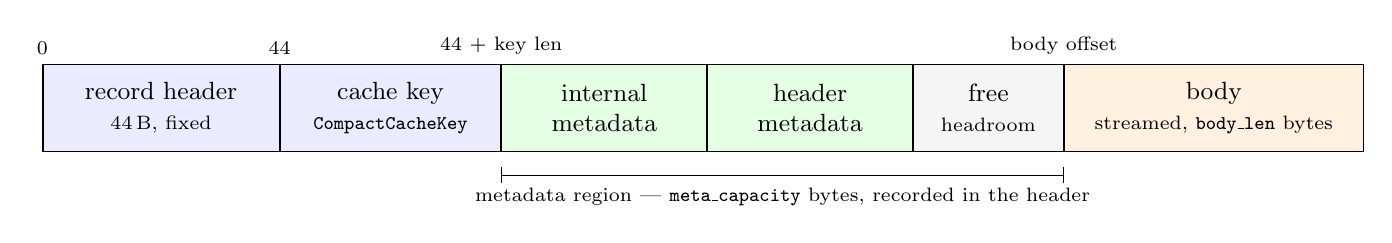
\begin{tikzpicture}[
          font=\small,
          seg/.style={draw, minimum height=11mm, align=center, anchor=west, inner sep=3pt},
        ]
        \node[seg, fill=blue!8,    minimum width=30mm] (hdr) at (0,0)      {record header\\{\scriptsize 44\,B, fixed}};
        \node[seg, fill=blue!8,    minimum width=28mm] (key) at (hdr.east) {cache key\\{\scriptsize\ttfamily CompactCacheKey}};
        \node[seg, fill=green!10,  minimum width=26mm] (im)  at (key.east) {internal\\metadata};
        \node[seg, fill=green!10,  minimum width=26mm] (hm)  at (im.east)  {header\\metadata};
        \node[seg, fill=gray!8,    minimum width=19mm] (fr)  at (hm.east)  {free\\{\scriptsize headroom}};
        \node[seg, fill=orange!12, minimum width=38mm] (bd)  at (fr.east)  {body\\{\scriptsize streamed, \texttt{body\_len} bytes}};
        \node[font=\scriptsize, anchor=south] at (hdr.north west) {0};
        \node[font=\scriptsize, anchor=south] at (key.north west) {44};
        \node[font=\scriptsize, anchor=south] at (im.north west)  {44 + key len};
        \node[font=\scriptsize, anchor=south] at (bd.north west)  {body offset};
        \draw[{Bar}-{Bar}] ([yshift=-3mm]im.south west) -- node[below=1pt, font=\scriptsize]{metadata region --- \texttt{meta\_capacity} bytes, recorded in the header} ([yshift=-3mm]fr.south east);
      \end{tikzpicture}
      \end{adjustbox}
      \caption{The record's segments in file order.}\label{dsn:singlefile-strip}
    \end{subfigure}

    \medskip

    \begin{subfigure}{\textwidth}
      \centering
      \begin{adjustbox}{max width=0.85\textwidth}
      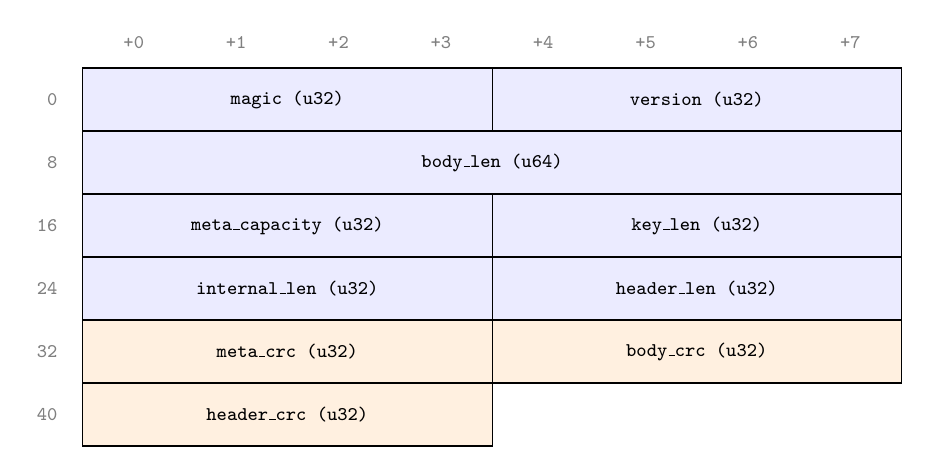
\begin{tikzpicture}[x=13mm, y=8mm, font=\ttfamily\scriptsize]
        \foreach \c in {0,...,7} {\node[gray] at (\c+0.5, 0.4) {+\c};}
        \foreach \r/\o in {0/0, 1/8, 2/16, 3/24, 4/32, 5/40}
          {\node[gray, anchor=east] at (-0.15, -\r-0.5) {\o};}
        \draw[fill=blue!8]    (0,-1) rectangle (4,0);   \node at (2,-0.5) {magic (u32)};
        \draw[fill=blue!8]    (4,-1) rectangle (8,0);   \node at (6,-0.5) {version (u32)};
        \draw[fill=blue!8]    (0,-2) rectangle (8,-1);  \node at (4,-1.5) {body\_len (u64)};
        \draw[fill=blue!8]    (0,-3) rectangle (4,-2);  \node at (2,-2.5) {meta\_capacity (u32)};
        \draw[fill=blue!8]    (4,-3) rectangle (8,-2);  \node at (6,-2.5) {key\_len (u32)};
        \draw[fill=blue!8]    (0,-4) rectangle (4,-3);  \node at (2,-3.5) {internal\_len (u32)};
        \draw[fill=blue!8]    (4,-4) rectangle (8,-3);  \node at (6,-3.5) {header\_len (u32)};
        \draw[fill=orange!12] (0,-5) rectangle (4,-4);  \node at (2,-4.5) {meta\_crc (u32)};
        \draw[fill=orange!12] (4,-5) rectangle (8,-4);  \node at (6,-4.5) {body\_crc (u32)};
        \draw[fill=orange!12] (0,-6) rectangle (4,-5);  \node at (2,-5.5) {header\_crc (u32)};
      \end{tikzpicture}
      \end{adjustbox}
      \caption{The 44-byte record header: fixed-width little-endian fields at
        naturally aligned offsets (row offsets left, byte positions above), so
        the block round-trips between disk and a \texttt{\#[repr(C)]} struct
        without repacking.}\label{dsn:singlefile-header}
    \end{subfigure}
    \caption{Object-file record layout: the on-disk structure of one cache
      object. Its self-delimiting fields are also what would let a future
      version reuse it, unchanged, inside an aggregate file
      (\reqref{ADR-EFFICIENCY.COMPACTION-01}).}\label{dsn:singlefile-layout}
  \end{figure}

  \textit{Basis: \pgsrc{pingora-cache/src/memory.rs}{38}{\texttt{MemCache}'s
  per-object metadata pair \texttt{BinaryMeta = (Vec<u8>, Vec<u8>)}} and its
  \pgsrc{pingora-cache/src/memory.rs}{45}{\texttt{TempObject}} (in-memory
  tracking of an in-flight write's valid length);
  \pgsrc{pingora-cache/src/meta.rs}{890}{\texttt{CacheMeta::serialize}} /
  \pgsrc{pingora-cache/src/meta.rs}{898}{\texttt{deserialize(internal,
  header)}}; internal-metadata fields per
  \pgsrc{pingora-cache/src/meta.rs}{83}{\texttt{InternalMetaV2}}.}

  \reqdiaglink{global}{\textit{View complete diagram.}}

  \reqexpect{refine}{SDS-LAYOUT.KEYSEGMENT-01}{Specify the key segment's
  byte encoding --- its fields' order and sizes, how the presence of a
  variance hash is marked, and how the tag is delimited --- so that each key
  has exactly one encoding.}
  \reqexpect{verify}{TC-LAYOUT.OBJECTFILE-01}{Verify that a reader accepts a
  record only when its magic, version, header and metadata CRCs, and stored
  key all validate, its metadata segments fit its capacity, its body offset
  lies within the file, and the file's length is exactly the
  computed body offset plus body_len; that any single violation is a miss
  and leaves the file in place; that a body whose checksum mismatches is read
  to a normal end, and is logged when the read-time check is on; and that a
  metadata read racing an in-place update returns one complete version.}
  \reqcover{satisfy}{IMP}

  \refine{ADR-STORAGE.OBJECTFILE-01}
  \refine{ADR-PERSISTENCE.DURABILITY-01}
  \satisfy{FRE-COMPAT.FORMATUPGRADE-01}
  \satisfy{FRE-COMPLIANCE.INCOMPLETE-01}
  \satisfy{FRE-COMPLIANCE.HEADERS-01}
  \satisfy{FRE-COMPLIANCE.FRESHNESS-01}
  \satisfy{FRE-COMPLIANCE.VALIDATORS-01}
  \satisfy{FRE-COMPLIANCE.BODY-01}
  \satisfy{FRE-COMPLIANCE.TRAILERS-01}
  \trace{FDS-STORAGE.PUBLISH-01}
  \trace{FDS-STORAGE.METAUPDATE-01}
  \trace{ADR-EFFICIENCY.COMPACTION-01}
  \trace{FRE-COMPLIANCE.REVALIDATION-01}
  \trace{FRE-COMPAT.EVICTION-01}
  \trace{FRE-COMPAT.STREAMING-01}
  \trace{FDS-EVICTION.STARTUP-01}
  \trace{SDS-LAYOUT.SHARDING-01}

\end{requirement}

\begin{requirement}{SDS-LAYOUT.KEYSEGMENT-01}[draft][structuralRequirement]{Key segment encoding}

  \localreqdiagram*{dsn3}{\reqid}{\reqdesc}

  The key segment of a record (\reqref{SDS-LAYOUT.OBJECTFILE-01}) holds the
  object's
  \texttt{CompactCacheKey}\footnote{\pgsrc{pingora-cache/src/key.rs}{153}{\texttt{CompactCacheKey}}.}
  as these fields, in this order, with no padding between them:
  \begin{itemize}
    \item \texttt{primary} (16 bytes): the key's primary hash.
    \item The \emph{variance flag} (1 byte): 1 when a variance hash follows,
      0 when none does.
    \item \texttt{variance} (16 bytes): the key's variance hash, present
      exactly when the variance flag is 1.
    \item \texttt{user\_tag}: the tag's UTF-8 bytes, filling the rest of the
      segment.
  \end{itemize}
  Both hashes are
  \texttt{HashBinary}\footnote{\pgsrc{pingora-cache/src/key.rs}{26}{\texttt{HashBinary}}
  is a \texttt{[u8; 16]}.} values. The tag carries no length of its own: the
  header's \texttt{key\_len} bounds the segment, so whatever follows the
  fixed fields is the tag. Each key therefore has exactly one encoding, which
  is what lets a reader compare a stored key with the key it looked up byte
  for byte.

  Only the restart-time scan decodes a stored key, to rebuild the
  \texttt{CompactCacheKey} it admits to the eviction manager
  (\reqref{FDS-EVICTION.STARTUP-01}). IF a key segment is shorter than the
  fields its variance flag announces, carries a variance flag other than 0 or
  1, or holds a tag that is not valid UTF-8, THEN the restart-time scan shall
  reclaim the record as damaged (\reqref{FDS-STORAGE.RECLAIM-01}).

  The field sizes are part of the record format: a \texttt{pingora-cache}
  release that changed the size of \texttt{HashBinary} would change what is
  stored, and so would require a new format version
  (\reqref{FRE-COMPAT.FORMATUPGRADE-01}).

  \reqdiaglink{global}{\textit{View complete diagram.}}

  \reqexpect{verify}{TC-LAYOUT.KEYSEGMENT-01}{Verify that keys with and
  without a variance hash, and with an empty and a non-empty tag, encode to
  the specified layout and decode back to themselves; that a segment too
  short for its fields, a variance flag other than 0 or 1, and a tag that is
  not UTF-8 are each rejected; and that the restart-time scan reclaims a
  record whose key does not decode.}
  \reqcover{satisfy}{IMP}

  \refine{SDS-LAYOUT.OBJECTFILE-01}
  \trace{FDS-EVICTION.STARTUP-01}
  \trace{FDS-STORAGE.RECLAIM-01}
  \trace{FRE-COMPAT.FORMATUPGRADE-01}
\end{requirement}


\begin{requirement}{FDS-EVICTION.STARTUP-01}[draft][functionalRequirement]{Startup: reconstruction procedure}

  \localreqdiagram*{fdsstartup01}{\reqid}{\reqdesc}

  \textbf{A dedicated API, not raw primitives.} The \texttt{Storage} trait
  has no startup lifecycle hook, so this reconstruction is orchestrated by
  \emph{Eviction Recovery}: a distinct API surface in the same crate as the
  \texttt{Storage} implementation, additional to it rather than folded into
  it, and --- unlike \texttt{CacheLock} or the \texttt{EvictionManager}
  itself --- never invoked \emph{per request}: it is called once per process
  start, possibly after serving has already begun. Exposing only primitives
  instead (enumerate persisted entries, an \texttt{admit} passthrough) would
  force every integrator to reimplement the same scan-and-reconcile
  sequencing below, and doing so from outside the crate would mean exposing
  the private on-disk object-record format this specification keeps
  internal everywhere else (\reqref{SDS-LAYOUT.OBJECTFILE-01}); folding it
  into a custom \texttt{EvictionManager} was already ruled out by
  \reqref{ADR-COMPAT.EVICTION-01}, which adopted the stock manager
  specifically to avoid building one. The cost is a second public API
  surface beyond \texttt{Storage}, with its own contract to document and
  version --- but a single one, safe to call unconditionally whether a
  first launch, a post-crash restart, or the new side of a hot upgrade
  (\reqref{FRE-COMPAT.HOTUPGRADE-01}): with no shutdown hook and no
  snapshot, there is nothing to call at the wrong time or to poison during
  a drain.

  \textbf{The procedure.} At process start, Eviction Recovery's
  \texttt{recover()} shall reconstruct the eviction manager from the published
  records, per \reqref{ADR-COMPAT.EVICTION-01}. On the incoming side of a hot
  upgrade the integrator calls it only once its server holds the listening
  sockets and the upgrade's close timeout has elapsed
  (\reqref{FDS-COMPAT.READONLY-01}). \texttt{recover()} enumerates the tree
  (\reqref{ADR-PERSISTENCE.MECHANISM-01}), classifying each entry as
  \reqref{FDS-STORAGE.RECLAIM-01} specifies, and admits every record it keeps
  with \texttt{admit(entry key, size, fresh\_until)}, where the entry key is the
  record's own \texttt{CompactCacheKey} carried in a \texttt{CacheEntryKey} with
  no entry identifier (\reqref{ADR-COMPAT.ENTRYID-01}) --- the same shape
  \texttt{HttpCache} builds for a live admission, so the two paths address one
  entry rather than two --- and \texttt{size} is the
  record size --- the file's length --- the same size a completed store
  reports (\reqref{FDS-STORAGE.PUBLISH-01}). Each \texttt{admit} may return
  eviction victims --- the manager deducts their sizes immediately and
  expects the caller to remove them from storage --- so the procedure shall
  purge every returned victim from \texttt{Storage} as an eviction, naming it by
  the exact entry the manager returned (\texttt{PurgeTarget::Exact}), exactly
  as \texttt{HttpCache} does after a live admission; a store found over its
  budget at startup is thereby brought back under it. Once the backend is
  read-only (\reqref{FDS-COMPAT.READONLY-01}), the procedure shall stop: it
  reads no further entry, and skips its remaining admissions and ghost-entry
  checks, since the eviction manager they would update is discarded when the
  process exits. It shall stop the same way, run by the hot-upgrade
  helper's recovery service, once the server starts shutting down
  (\reqref{FDS-COMPAT.READONLY-01}). \texttt{recover()}
  returns once enumeration and the reconciliation below have completed; that
  return is the backend reporting its restart procedure complete
  (\reqref{FRE-COMPAT.EVICTION-01}).

  \textbf{Running alongside live traffic.} Whether the integrator starts
  serving before \texttt{recover()} returns is its own choice
  (\reqref{ADR-COMPAT.EVICTION-01}). The manager keys entries by
  \texttt{CacheEntryKey}, which for this backend carries the
  \texttt{CompactCacheKey} and nothing more, so the scan and live traffic
  admitting the same object update one entry rather than duplicating it. The procedure shall
  close the races the decision identifies, each by acting while holding the
  key's publication lock (\reqref{FDS-STORAGE.METAUPDATE-01}), which a live
  store's rename also takes before that store is admitted:
  \begin{itemize}
    \item \emph{Stale size.} Immediately before admitting a record, the
      procedure re-checks its path under the lock. If the path is gone or
      now refers to a different file than the one read, it skips the record
      --- live traffic removed it, or published and will admit its
      replacement; otherwise it admits the record with the file's current
      length while still holding the lock.
    \item \emph{Ghost entries.} After enumeration, for every key it admitted,
      the procedure checks under the lock whether the canonical path still
      exists, and calls the manager's \texttt{remove} --- which takes the
      borrowed \pgsrc{pingora-cache/src/eviction/mod.rs}{169}{\texttt{CacheEntryKeyRef}}
      form of the same identity --- for any that does not.
      A key live traffic republishes after that check is admitted by the live
      path afterwards.
  \end{itemize}
  An object live traffic has just read may still come back from an
  \texttt{admit} as a victim; it is purged like any other, and accounting
  stays exact.

  \begin{figure}[H]
    \centering
    \begin{adjustbox}{max width=\textwidth}
    \begin{sequencediagram}
      \newinst[0.0]{Startup}{\guillemotleft actor\guillemotright\ Startup}
      \newinst[0.5]{EvictionRecovery}{Eviction Recovery}
      \newinst[5.4]{EvictionManager}{EvictionManager}
      \newinst[0.5]{Storage}{Storage}
      \newinst[0.5]{HttpCache}{HttpCache}
      \begin{sdalt}{par}{[timing is the integrator's choice]}
        \begin{call}{Startup}{recover()}{EvictionRecovery}{}
          \begin{call}{EvictionRecovery}{enumerate()}{Storage}{entries}
          \end{call}
          \begin{call}{EvictionRecovery}{admit(entry key, size, fresh\_until)}{EvictionManager}{victims}
          \end{call}
          \begin{call}{EvictionRecovery}{purge(Exact(victim), Eviction) (for each victim)}{Storage}{}
          \end{call}
          \begin{call}{EvictionRecovery}{remove(entry key) for each admitted key now absent}{EvictionManager}{}
          \end{call}
        \end{call}
      \sdpart{[begin serving, whenever chosen]}
        \begin{call}{Startup}{begin serving}{HttpCache}{}
          \begin{call}{HttpCache}{admit / access (live)}{EvictionManager}{}
          \end{call}
        \end{call}
      \end{sdalt}
    \end{sequencediagram}
    \end{adjustbox}
    \caption{Startup reconstruction, carried out by Eviction Recovery (\texttt{Storage} and the \texttt{EvictionManager} never call each other). \texttt{Startup} --- the integrator's own code --- independently calls \texttt{recover()} and, on its own schedule, tells \texttt{HttpCache} to begin serving; if serving starts before reconstruction finishes, live \texttt{HttpCache} traffic touches the \texttt{EvictionManager} in parallel with the scan.}\label{fig:fds-startup-seq}
  \end{figure}

  \reqdiaglink{global}{\textit{View complete diagram.}}

  \reqexpect{verify}{TC-EVICTION.RECONSTRUCT-01}{Verify that when recover()
  returns the manager holds exactly the published set with record sizes,
  including when stores, replacements, and purges run during the scan, and
  that no snapshot or delta log is read or written at any point.}
  \reqcover{satisfy}{IMP}

  \refine{ADR-COMPAT.EVICTION-01}
  \trace{ADR-PERSISTENCE.MECHANISM-01}
  \trace{FDS-COMPAT.READONLY-01}
  \trace{FDS-STORAGE.RECLAIM-01}
  \satisfy{FRE-COMPAT.EVICTION-01}
  \satisfy{FRE-COMPAT.HOTUPGRADE-01}
\end{requirement}

\begin{requirement}{FDS-COMPAT.READONLY-01}[draft][functionalRequirement]{Read-only on the upgrade signal}

  \localreqdiagram*{fdsreadonly01}{\reqid}{\reqdesc}

  \textbf{The read-only operation.} The backend shall expose a
  \texttt{set\_read\_only} operation, callable from any thread and
  idempotent, which the integrator calls when its server's execution-phase
  broadcast announces
  \texttt{GracefulUpgradeTransferringFds}.\footnote{\pgsrc{pingora-core/src/server/mod.rs}{235}{\texttt{Server::watch\_execution\_phase}}
  subscribes to the broadcast, which sends that phase when the upgrade signal
  arrives (\pgsrc{pingora-core/src/server/mod.rs}{279}{L279}).} A graceful
  terminate, which announces \texttt{GracefulTerminate} instead, does not
  call it: no incoming process will take over the cache, so stores that
  complete while sessions drain should still be published.

  \textbf{The read-only gate.} The backend shall keep a process-wide
  \emph{read-only} flag behind a read--write gate. Every durable change ---
  a store's final rename (\reqref{FDS-STORAGE.PUBLISH-01}), a purge's unlink
  (\reqref{FDS-STORAGE.PURGE-01}), either path of a metadata update
  (\reqref{FDS-STORAGE.METAUPDATE-01}) or of an expiry
  (\reqref{FDS-STORAGE.EXPIRE-01}), and a reclaim unlink
  (\reqref{FDS-STORAGE.RECLAIM-01}) --- holds the gate shared from the moment
  it checks the flag until the change is done. So does each of the restart
  scan's admission checks (\reqref{FDS-EVICTION.STARTUP-01}), which changes
  no file but takes a key's publication lock
  (\reqref{FDS-STORAGE.METAUPDATE-01}): every taker of that lock enters the
  gate first. \texttt{set\_read\_only} takes the gate exclusively to set the
  flag, so when it returns, nothing that entered the gate before it is still
  running, and nothing can enter afterwards.

  \textbf{Once read-only.} The process keeps draining its sessions; only its
  backend's changes to the shared cache stop. From then on the backend
  shall:
  \begin{itemize}
    \item keep opening stores and accepting their body writes, since failing
      to open a store would fail the client request that triggered
      it,\footnote{The proxy propagates the error from
      \pgsrc{pingora-proxy/src/proxy_cache.rs}{689}{\texttt{set\_miss\_handler}}
      with \texttt{?}.} and partial-hit readers inside this process
      (\reqref{FDS-STORAGE.PARTIAL-01}) keep streaming;
    \item in \texttt{finish}, remove the temporary instead of renaming it,
      while reporting the store created with its record size, so the request
      completes normally --- the entry this adds to the process's own
      eviction manager is discarded when the process exits;
    \item fail \texttt{purge} (of either purge type and either target kind),
      \texttt{expire}, and \texttt{update\_meta} with an error, changing nothing
      on disk;
    \item stop the restart scan, skipping any reclaim unlink and any
      admission check still pending --- the eviction manager the checks would
      update is discarded when the process exits;
    \item serve \texttt{lookup} and body reads unchanged.
  \end{itemize}

  \textbf{Ordering with the incoming process.} In the incoming process,
  Eviction Recovery's \texttt{recover()} (\reqref{FDS-EVICTION.STARTUP-01})
  shall start only after the server has taken over the listening sockets and a
  further \texttt{CLOSE\_TIMEOUT} (5~s) has elapsed, as
  \reqref{ADR-COMPAT.READONLY-01} decides. That wait is the one the outgoing
  process takes after handing over its listening sockets; since 0.9.0 the
  outgoing process skips it entirely when it had no sockets to send, which is
  not the hot-upgrade case this ordering is about. The takeover is complete once
  \texttt{Server::bootstrap} returns, or --- when bootstrap runs as a
  service --- once that service reports ready;\footnote{\pgsrc{pingora-core/src/server/mod.rs}{604}{\texttt{Server::bootstrap}}
  ``will try to get all its listening sockets in order to take them over'';
  \pgsrc{pingora-core/src/server/mod.rs}{612}{\texttt{bootstrap\_as\_a\_service}}
  runs the same work as a service, and a service started with dependencies
  waits for them to report ready
  (\pgsrc{pingora-core/src/server/mod.rs}{735}{L735}).} the server's
  \texttt{Running} phase is not a substitute, since the main loop announces it
  without waiting for a bootstrap service. The deliverable shall therefore
  run \texttt{recover()} as a background service that waits the close
  timeout before starting and, when bootstrap runs as a service, depends on
  that service; a direct \texttt{bootstrap} call takes the sockets over
  before any service starts. In a process started without the Pingora upgrade
  flag, which takes the sockets over from none, the service shall not wait.
  It shall provide that service and the
  \texttt{set\_read\_only} subscription together, as a helper that adds both
  to the integrator's server and takes the bootstrap service's handle when
  there is one, and document that hot upgrades require it. Once the server
  starts shutting down, the eviction manager the service fills is about to
  be discarded, so the service shall start no scan, and stop a running one
  at its next entry, as it stops for a read-only backend.

  \reqdiaglink{global}{\textit{View complete diagram.}}

  \reqcover{verify}{TC}
  \reqcover{satisfy}{IMP}

  \refine{ADR-COMPAT.READONLY-01}
  \satisfy{FRE-COMPAT.HOTUPGRADE-01}
  \trace{FRE-COMPLIANCE.PURGEDURABLE-01}
  \trace{FRE-COMPLIANCE.REVALIDATION-01}
\end{requirement}

